\begin{frame}{Materials and Methods}
\begin{block}{Pose estimation}
	\begin{itemize}
		\item Indoor - Vicon motion capture system
		\item Outdoor - Inertial Measurement Unit
	\end{itemize}

\begin{figure}
	\centering
	%\includegraphics[scale=0.15][trim={0 5mm 5mm 0},clip]{Figuras/new_bebop_vicon.jpg}
	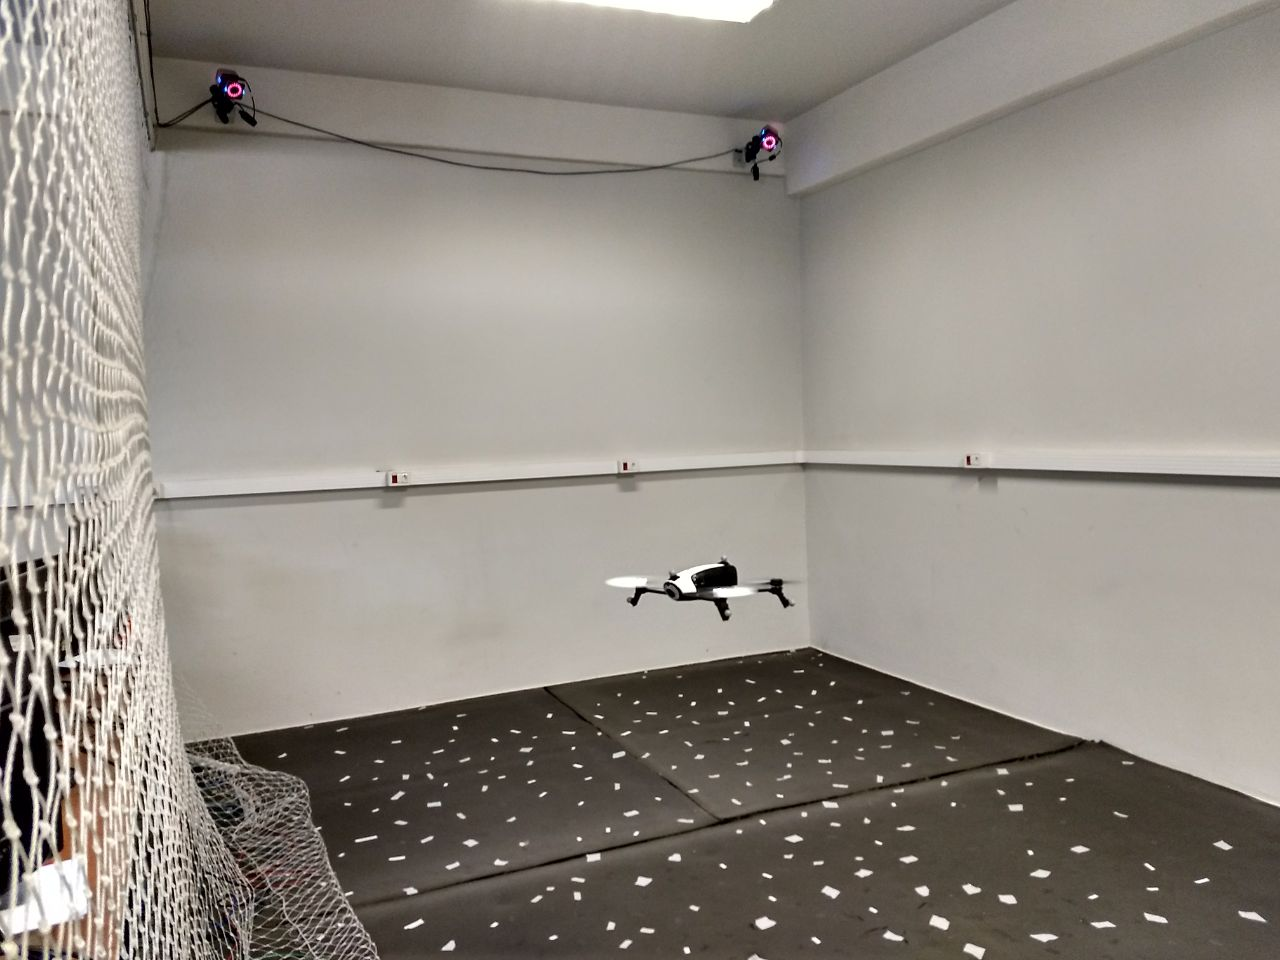
\includegraphics[clip,trim=0 0cm 0cm 0,width=6cm]{img/viconRoom.jpeg}
	%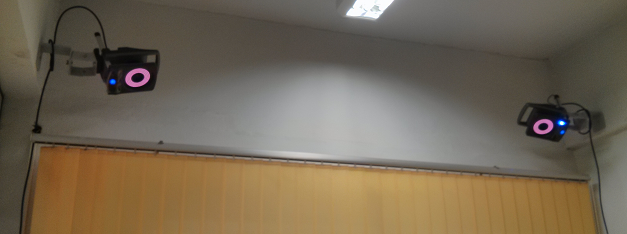
\includegraphics[scale=0.55]{Figuras/apendice1/camera_pos.png}
	\caption{A Vicon-T40S setup at the Intelligent Systems' Lab at USP in São Carlos}	\label{fig:camera_pos}
\end{figure}
\end{block}
\end{frame}

%%%%%%%%%%%%%%%%%%%%%%%%%%%%%%%% FRAME %%%%%%%%%%%%%%%%%%%%%%%%%%%%%%%%

\begin{frame}{Materials and Methods}
\begin{block}{Pose estimation}
\begin{figure}
	\centering
	\subfloat{
		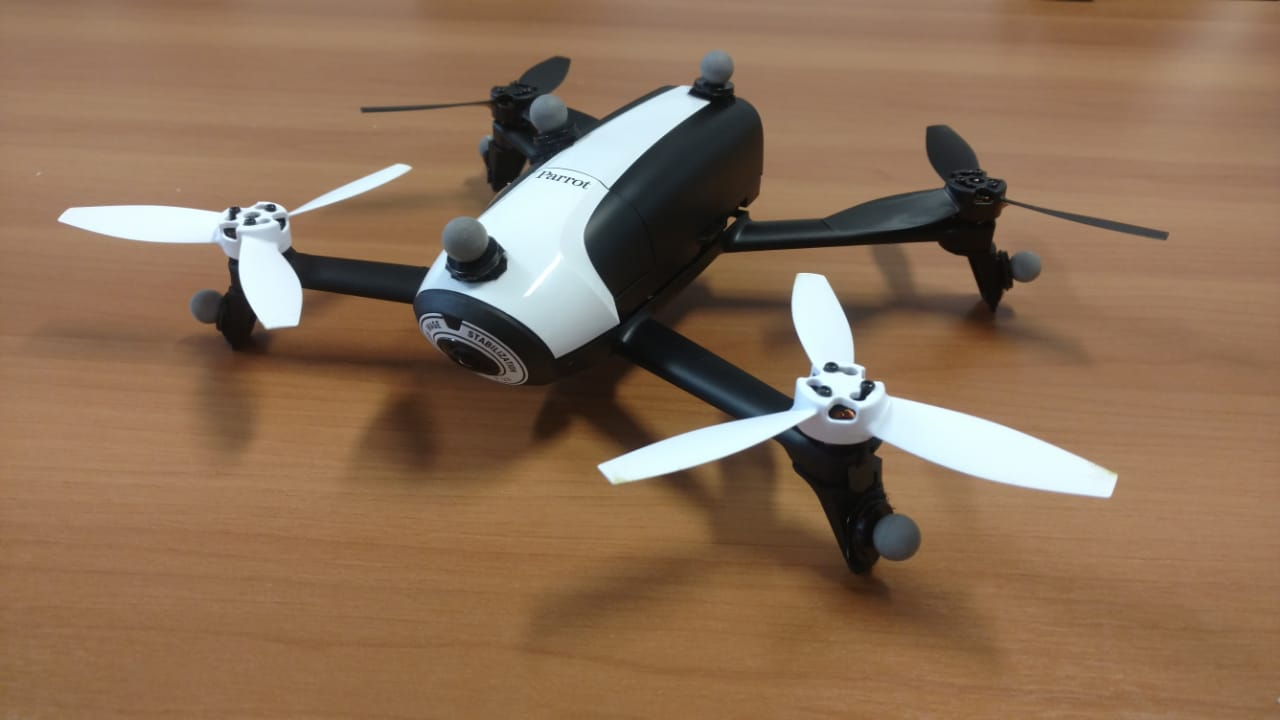
\includegraphics[clip,trim=1cm 2cm 2cm 0cm, width=4cm]{img/parrotMarcadores.jpeg}
	}
	\quad %espaco separador
	\subfloat{
		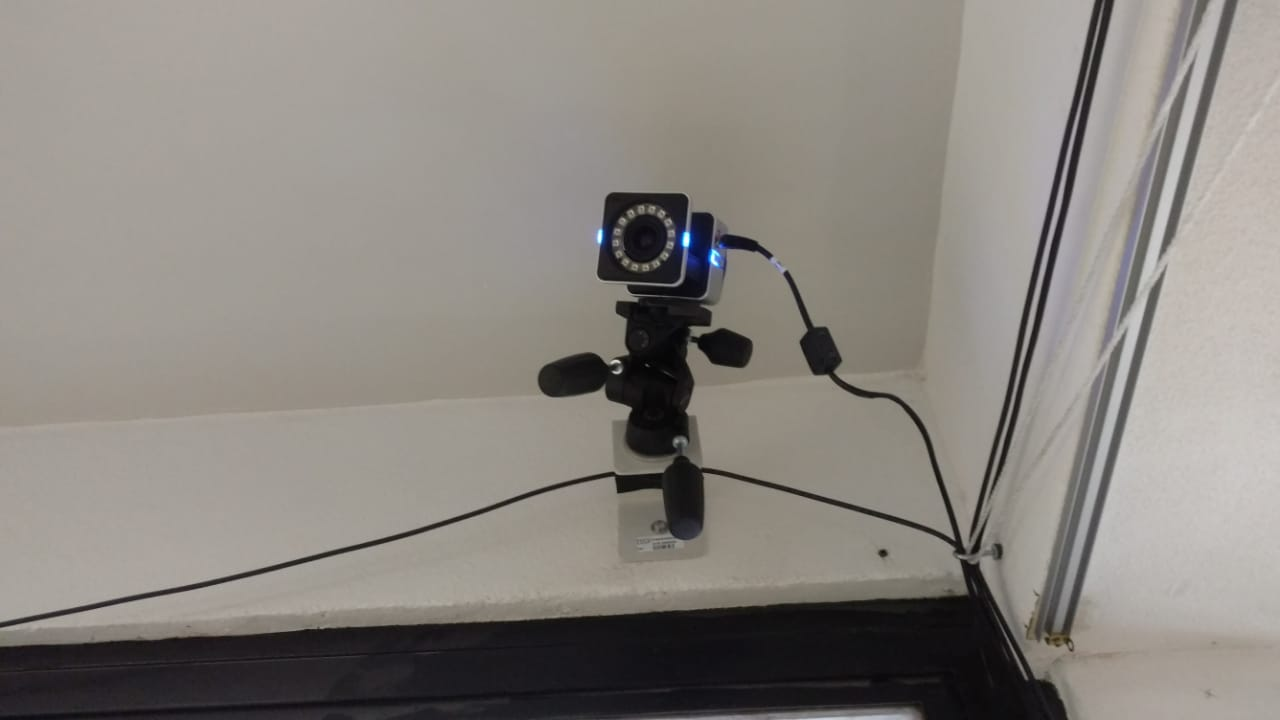
\includegraphics[clip,trim=0 0cm 0cm 0cm,width=4cm]{img/new_vicon1.jpg}
	} \\
	\subfloat{
		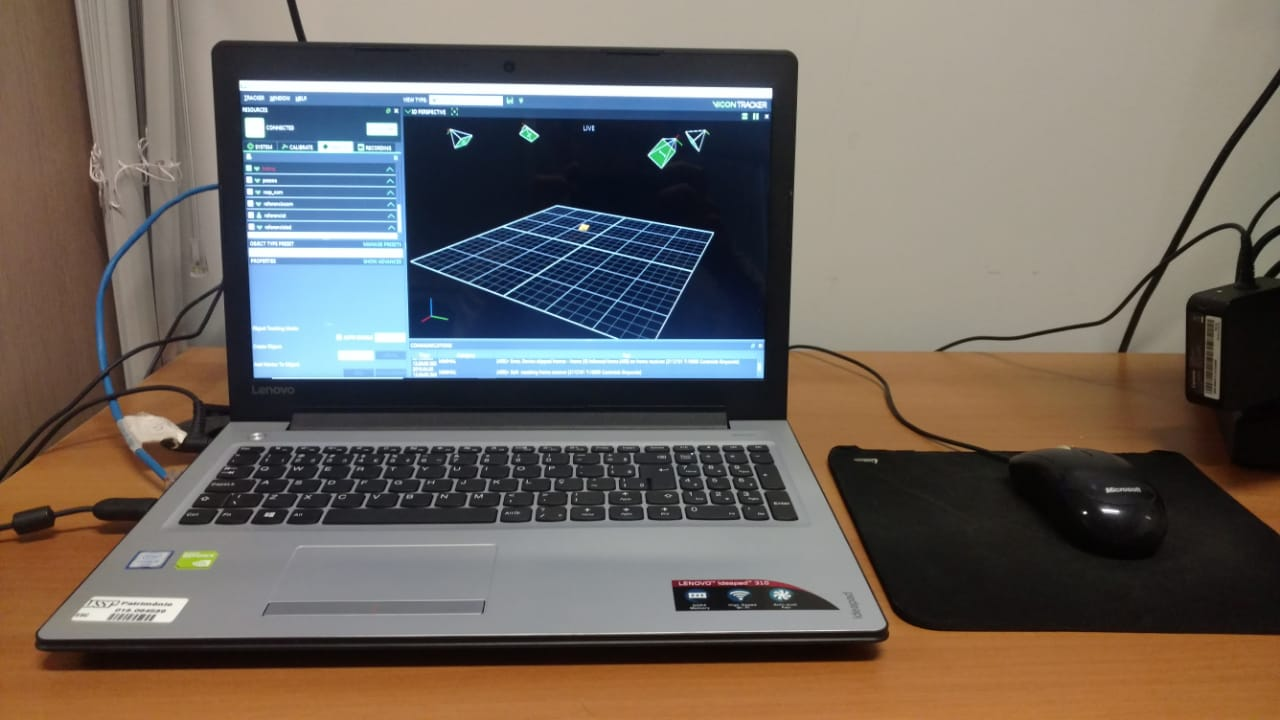
\includegraphics[width=4cm]{img/computador_vicon.jpg}
	}
	\quad %espaco separador
	\subfloat{
		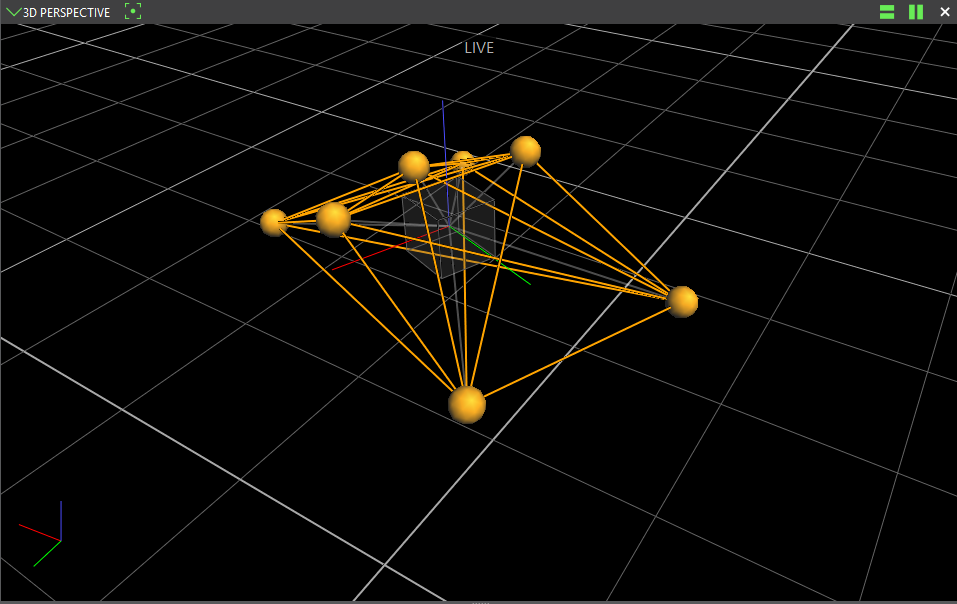
\includegraphics[width=4cm]{img/print_bebopTracker.png}
	}
\end{figure}
\end{block}
\end{frame}

%%%%%%%%%%%%%%%%%%%%%%%%%%%%%%%% FRAME %%%%%%%%%%%%%%%%%%%%%%%%%%%%%%%%

\begin{frame}{Materials and Methods}
\begin{block}{ROS-Based Platform}
\begin{itemize}
	\item Goal: Create an open source development environment for evaluating control strategies (UAVs and UGVs).
\end{itemize}

\begin{figure}[!h]
	\centering
	
\includegraphics[scale=0.5]{img/ros.png}
\end{figure}
\begin{itemize}
	\item ROS (Robot Operating System) provides libraries and tools to help software developers create robot applications.
	\item \textit{\textbf{drone\_dev}}: UAVs - Parrot Bebop 2
\end{itemize}
\end{block}

\end{frame}


%%%%%%%%%%%%%%%%%%%%%%%%%%%%%%%% FRAME %%%%%%%%%%%%%%%%%%%%%%%%%%%%%%%%

\begin{frame}{Materials and Methods}
\begin{block}{ROS-Based Platform - \textit{drone\_dev}}
\begin{figure}[!h]
	\centering
	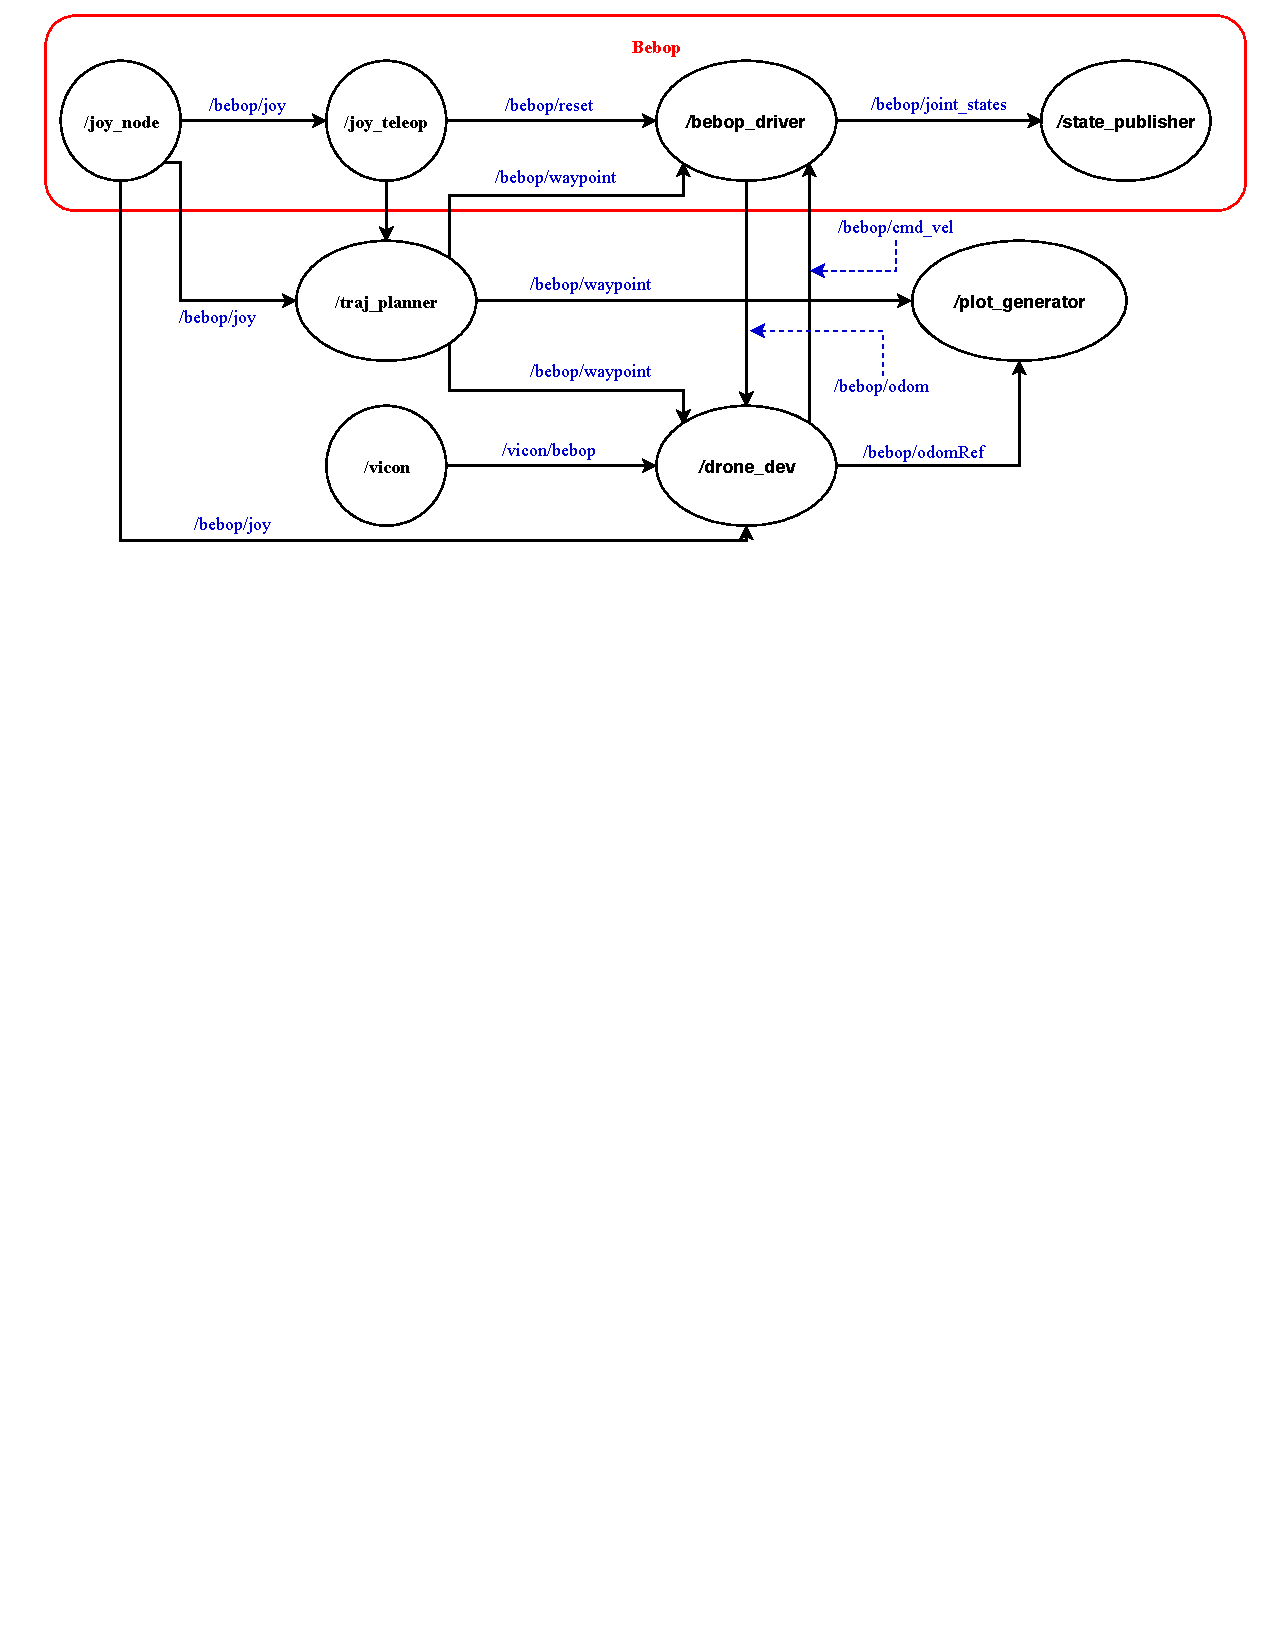
\includegraphics[scale=0.55,trim={0cm 18.5cm 0cm 0},clip]{img/rqtGraph01.pdf}
	\caption{Graph representation of the \textit{drone\_dev} system. Source: Author (2019)}\label{fig:rqtGraph}
\end{figure}
\end{block}
\end{frame}

%%%%%%%%%%%%%%%%%%%%%%%%%%%%%%%% FRAME %%%%%%%%%%%%%%%%%%%%%%%%%%%%%%%%

\begin{frame}{Materials and Methods}
\begin{block}{ROS-Based Platform - \textit{drone\_dev}}
\textbf{Main Features:}
\begin{itemize}
	\item Evaluate flight controller strategies:
	\begin{itemize}
		\item Proportional-Integral-Derivative
		\item Linear-Quadratic Regulator
		\item Feedback Linearization
		\item Robust Linear-Quadratic Regulator
	\end{itemize}
	\item Trajectory tracking reference
	\begin{itemize}
		\item Eight-shape (Gerono's Lemniscate)
		\item Circle in $xy$ plane
		\item Straight line 
	\end{itemize}
	\item Joystick for safety and guidance
	\item Kalman Filter for velocity estimation
\end{itemize}

\end{block}
\end{frame}

%%%%%%%%%%%%%%%%%%%%%%%%%%%%%%%% FRAME %%%%%%%%%%%%%%%%%%%%%%%%%%%%%%%%

\begin{frame}{Materials and Methods}
\begin{block}{ROS-Based Platform - \textit{drone\_dev}}

	\begin{figure}[!h]
	\centering
%	\begin{tikzpicture}
%	\begin{axis}[
%	legend columns=-1,
%	legend entries={R-LQR, Reference},
%	legend style={anchor = east},
%	legend to name=rlqrLegend,
%	ylabel={$\dot{x}(m/s)$},
%	xmin=6,xmax =40,
%	% ymin=-4,ymax =3,
%	ymin=-2,ymax =2,
%	xtick={0,5,10,15,20,25,30,35,40},
%	ytick={-2,0,2},
%	width=8cm,
%	height=2.5cm,
%	grid=major,]
%	\addplot [color=red] table [x=t2,y=ZsavedVelX]{KalmanXYZ.txt};
%	\addplot [color=blue, dashed, thick] table [x=t2,y=XsavedVelX]{KalmanXYZ.txt};
%	\end{axis}
%	\end{tikzpicture}\\
%	\begin{tikzpicture}
%	\begin{axis}[
%	ylabel={$\dot{y}(m/s)$},
%	width=8cm,
%	height=2.5cm,
%	xmin=6, xmax =40,
%	% ymin=-3,ymax =4,
%	ymin=-2,ymax =2,
%	xtick={0,5,10,15,20,25,30,35,40},
%	ytick={-2,0,2},
%	grid=major,]
%	\addplot [color=red] table [x=t2,y=ZsavedVelY]{KalmanXYZ.txt};
%	\addplot [color=blue, dashed, thick] table [x=t2,y=XsavedVelY]{KalmanXYZ.txt};
%	\end{axis}
%	\end{tikzpicture} \\
%	\begin{tikzpicture}
%	\begin{axis}[
%	legend columns=-1,
%	legend entries={Simple Differentiation, Kalman Filter},
%	legend to name=named1,
%	ylabel={$\dot{z}(m/s)$},
%	xlabel={$t(s)$},
%	xmin=6, xmax =40,
%	% ymin=-3,ymax =3,
%	ymin=-2,ymax =2,
%	width=8cm,
%	height=2.5cm,
%	xtick={0,5,10,15,20,25,30,35,40},
%	ytick={-2,0,2},
%	grid=major,]
%	\addplot [color=red] table [x=t2,y=ZsavedVelZ]{KalmanXYZ.txt};
%	\addplot [color=blue, dashed, thick] table [x=t2,y=XsavedVelZ]{KalmanXYZ.txt};
%	\end{axis}
%	\end{tikzpicture}
	\\
	\hspace{23pt} \ref{named1}
\end{figure}
\end{block}
\end{frame}

%%%%%%%%%%%%%%%%%%%%%%%%%%%%%%%% FRAME %%%%%%%%%%%%%%%%%%%%%%%%%%%%%%%%

\begin{frame}{Materials and Methods}
\begin{block}{ROS-Based Platform - \textit{drone\_dev}}
	\textbf{Testing Environment:}
	\begin{itemize}
		\item Host PC
		\begin{itemize}
			\item Intel Core i7-7700HQ 16GB
			\item Ubuntu 16.04 LTS
			\item ROS Kinect
			\item Eigen library
			\item \textit{bebop\_autonomy} and \textit{vicon\_bridge} 
		\end{itemize}
	\end{itemize}
		
	
\end{block}
\end{frame}

%%%%%%%%%%%%%%%%%%%%%%%%%%%%%%%% FRAME %%%%%%%%%%%%%%%%%%%%%%%%%%%%%%%%

\begin{frame}{Materials and Methods}
\begin{block}{ROS-Based Platform - \textit{drone\_dev}}
	\textbf{Testing Environment: Outdoor}
\begin{figure}[!h]
	\centering
	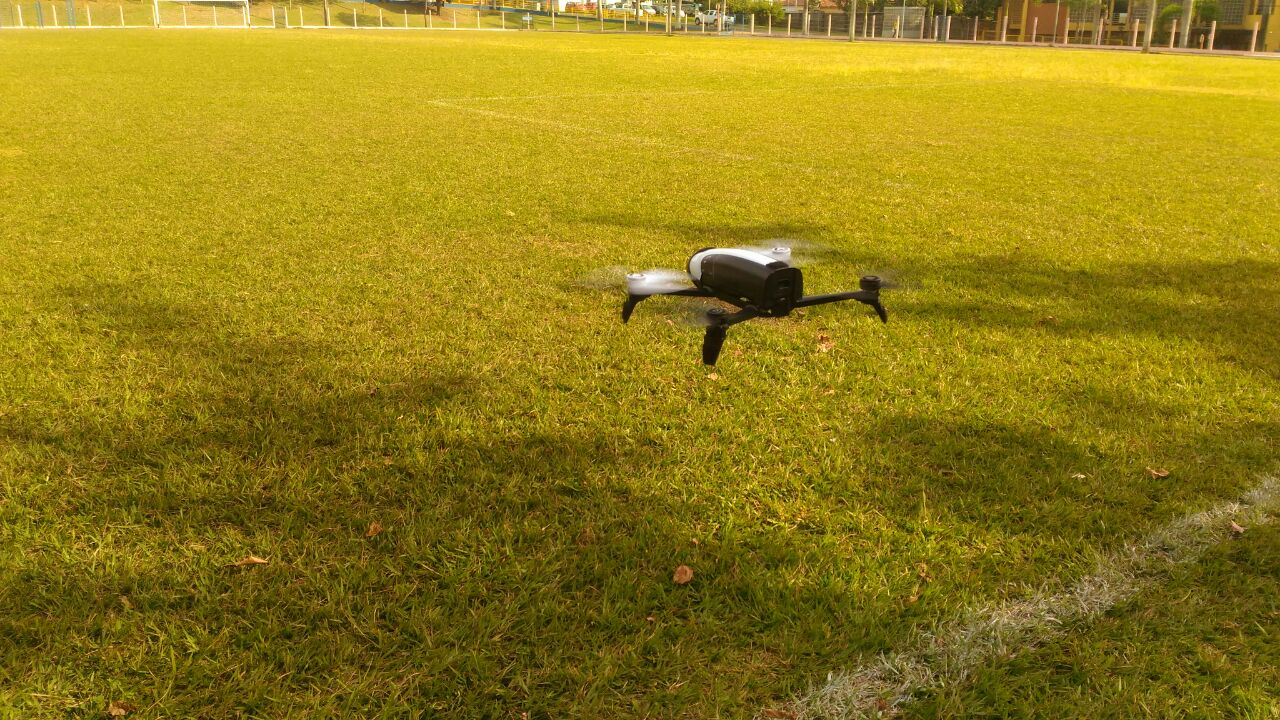
\includegraphics[width=5.5cm]{img/parrotOutdoor1.jpeg}
	\hspace{0.25cm}
	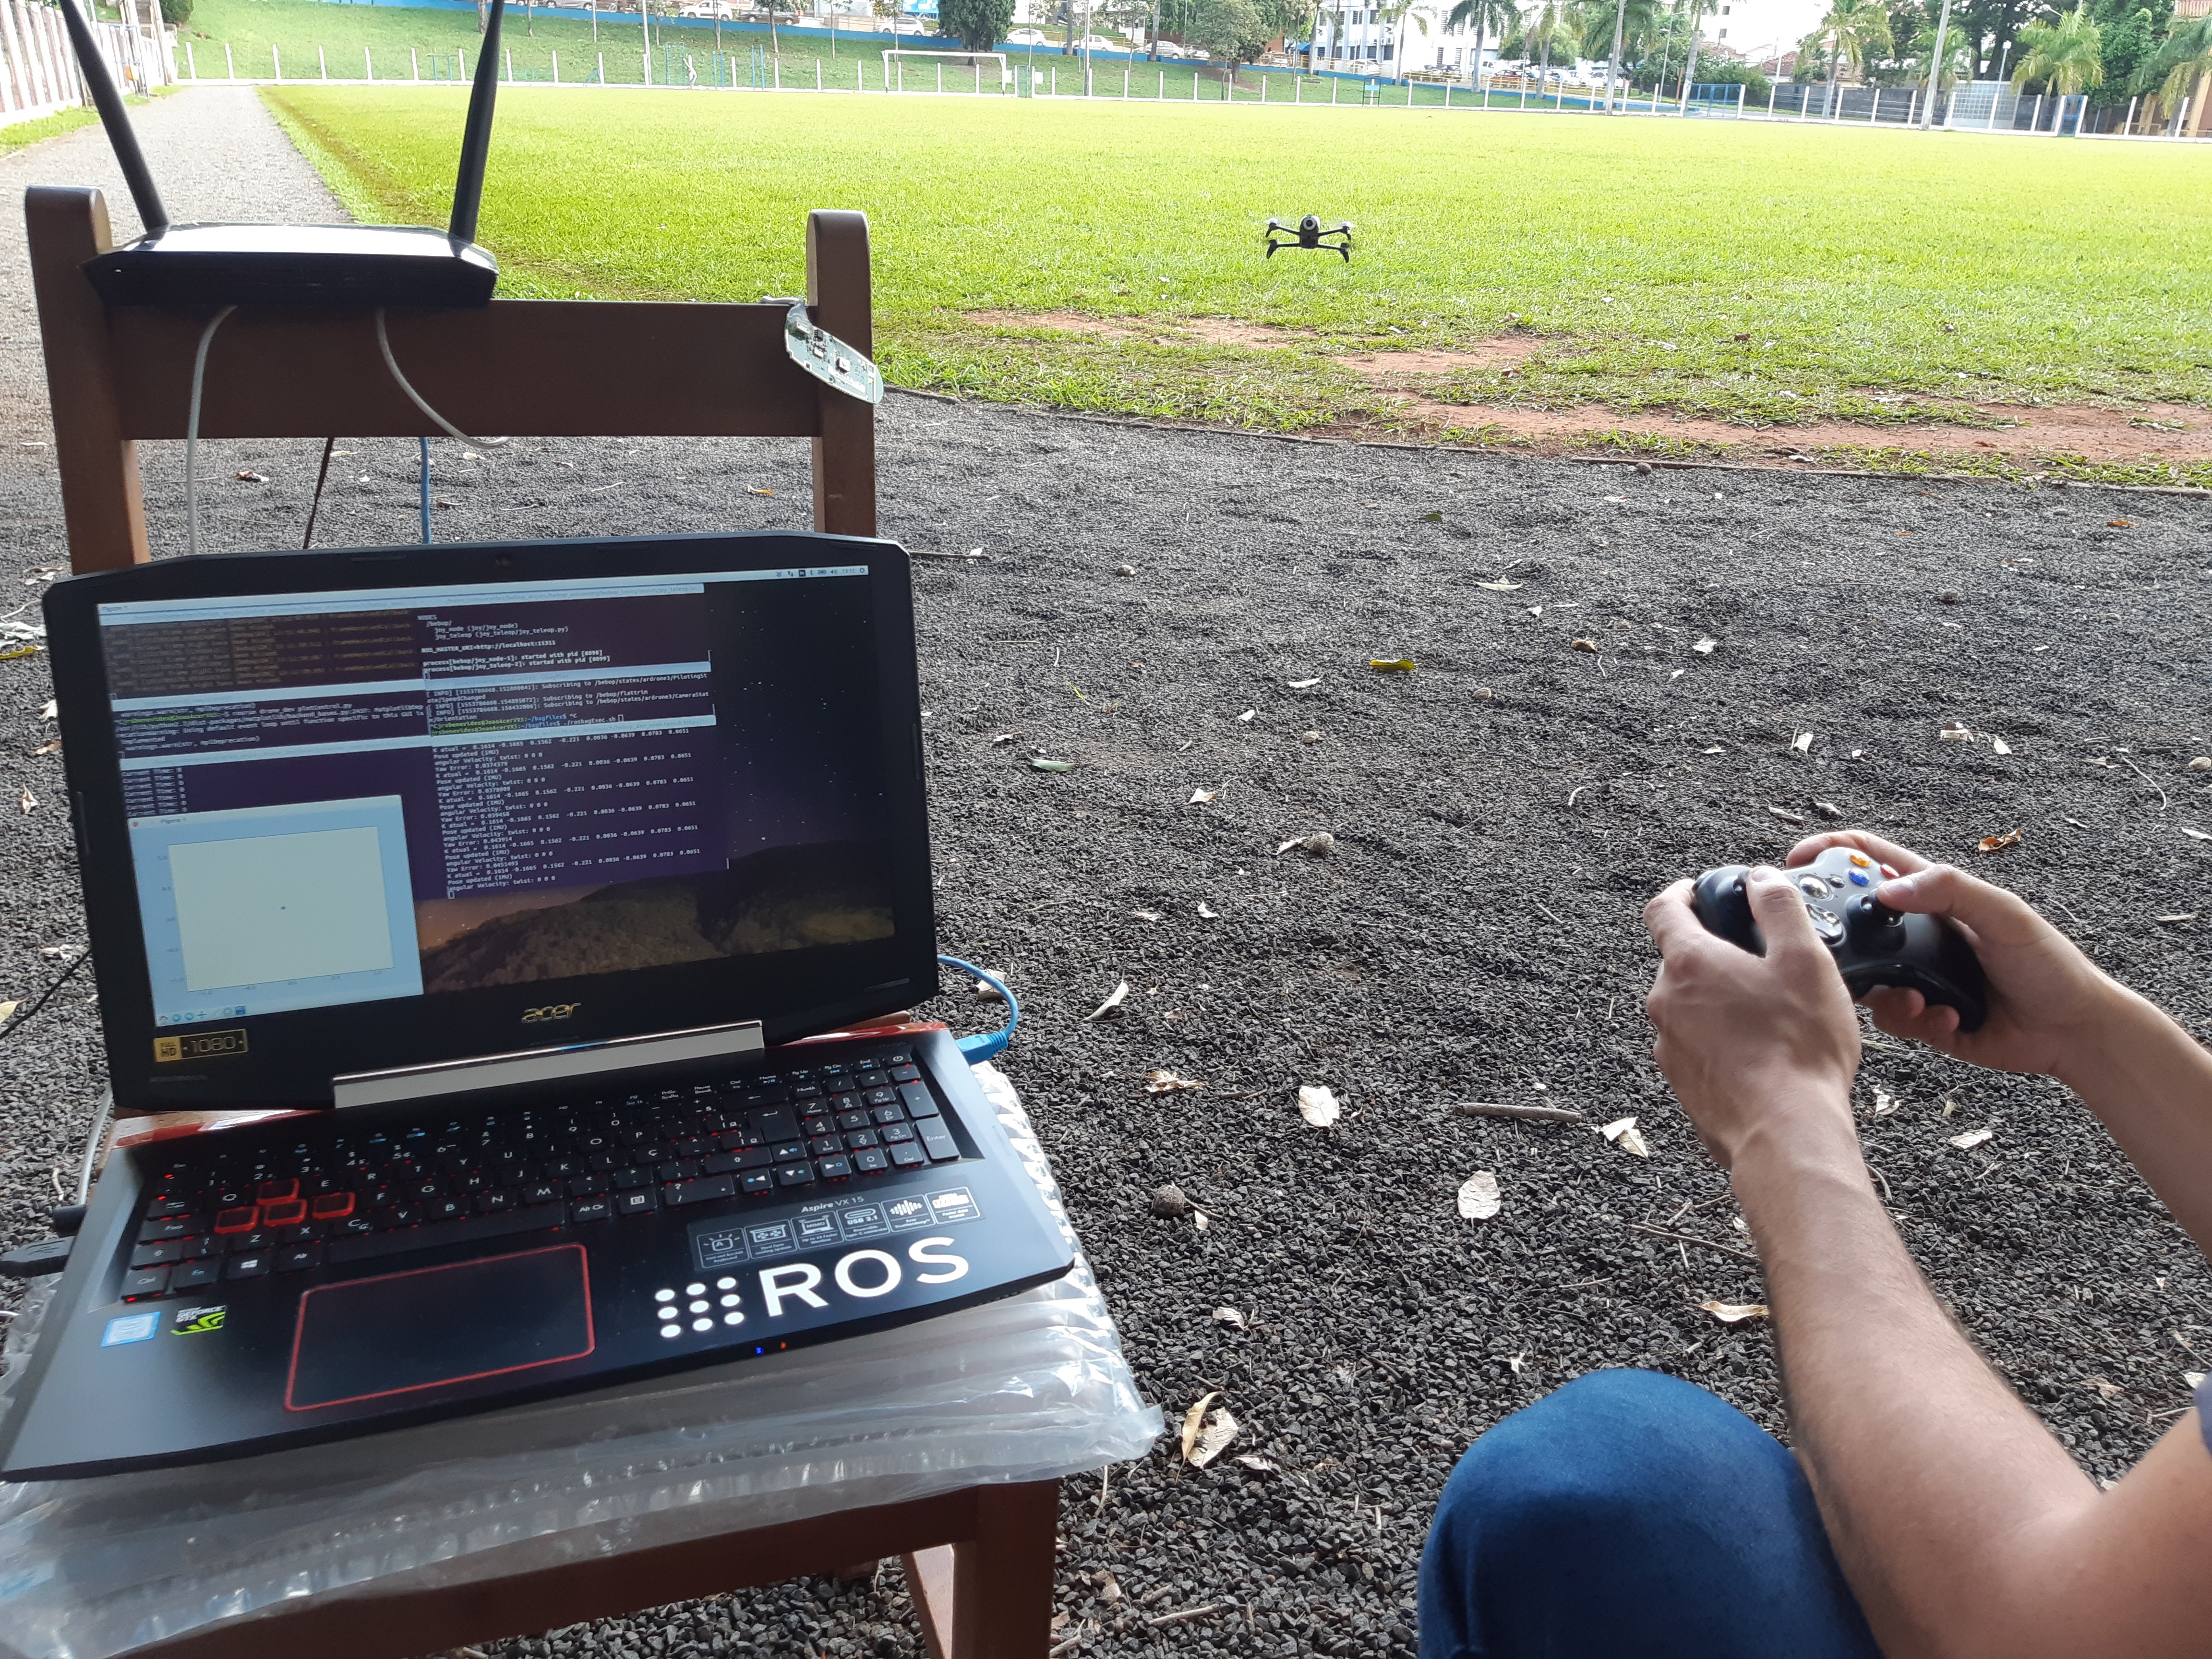
\includegraphics[width=5.5cm]{img/outdoorPC.jpg}
\end{figure}
	
	
\end{block}
\end{frame}

%%%%%%%%%%%%%%%%%%%%%%%%%%%%%%%% FRAME %%%%%%%%%%%%%%%%%%%%%%%%%%%%%%%%

\begin{frame}{Materials and Methods}
\begin{block}{ROS-Based Platform - \textit{drone\_dev}}
	\textbf{Testing Environment: Indoor}	
	\begin{figure}[!h]
		\centering
		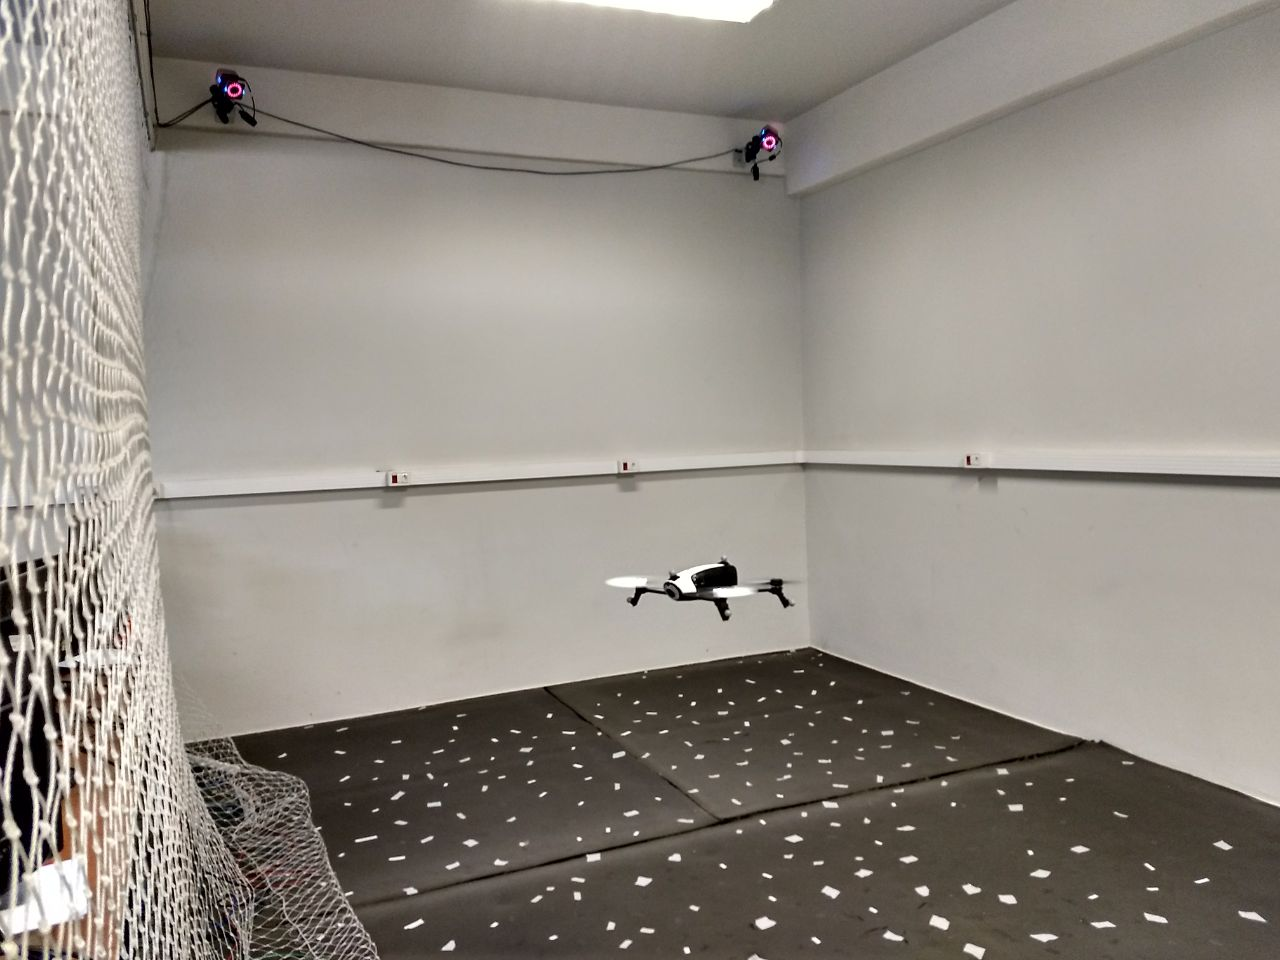
\includegraphics[scale=0.15]{img/viconRoom.jpeg}
		\caption{Drone arena at the Robotics Center in São Carlos. Source: Author (2019)}	\label{fig:viconRoom}
	\end{figure}
	
	
\end{block}
\end{frame}

%%%%%%%%%%%%%%%%%%%%%%%%%%%%%%%% FRAME %%%%%%%%%%%%%%%%%%%%%%%%%%%%%%%%

\begin{frame}{Materials and Methods}
\begin{block}{ROS-Based Platform - \textit{drone\_dev}}
	\begin{figure}[!h]
		\centering
		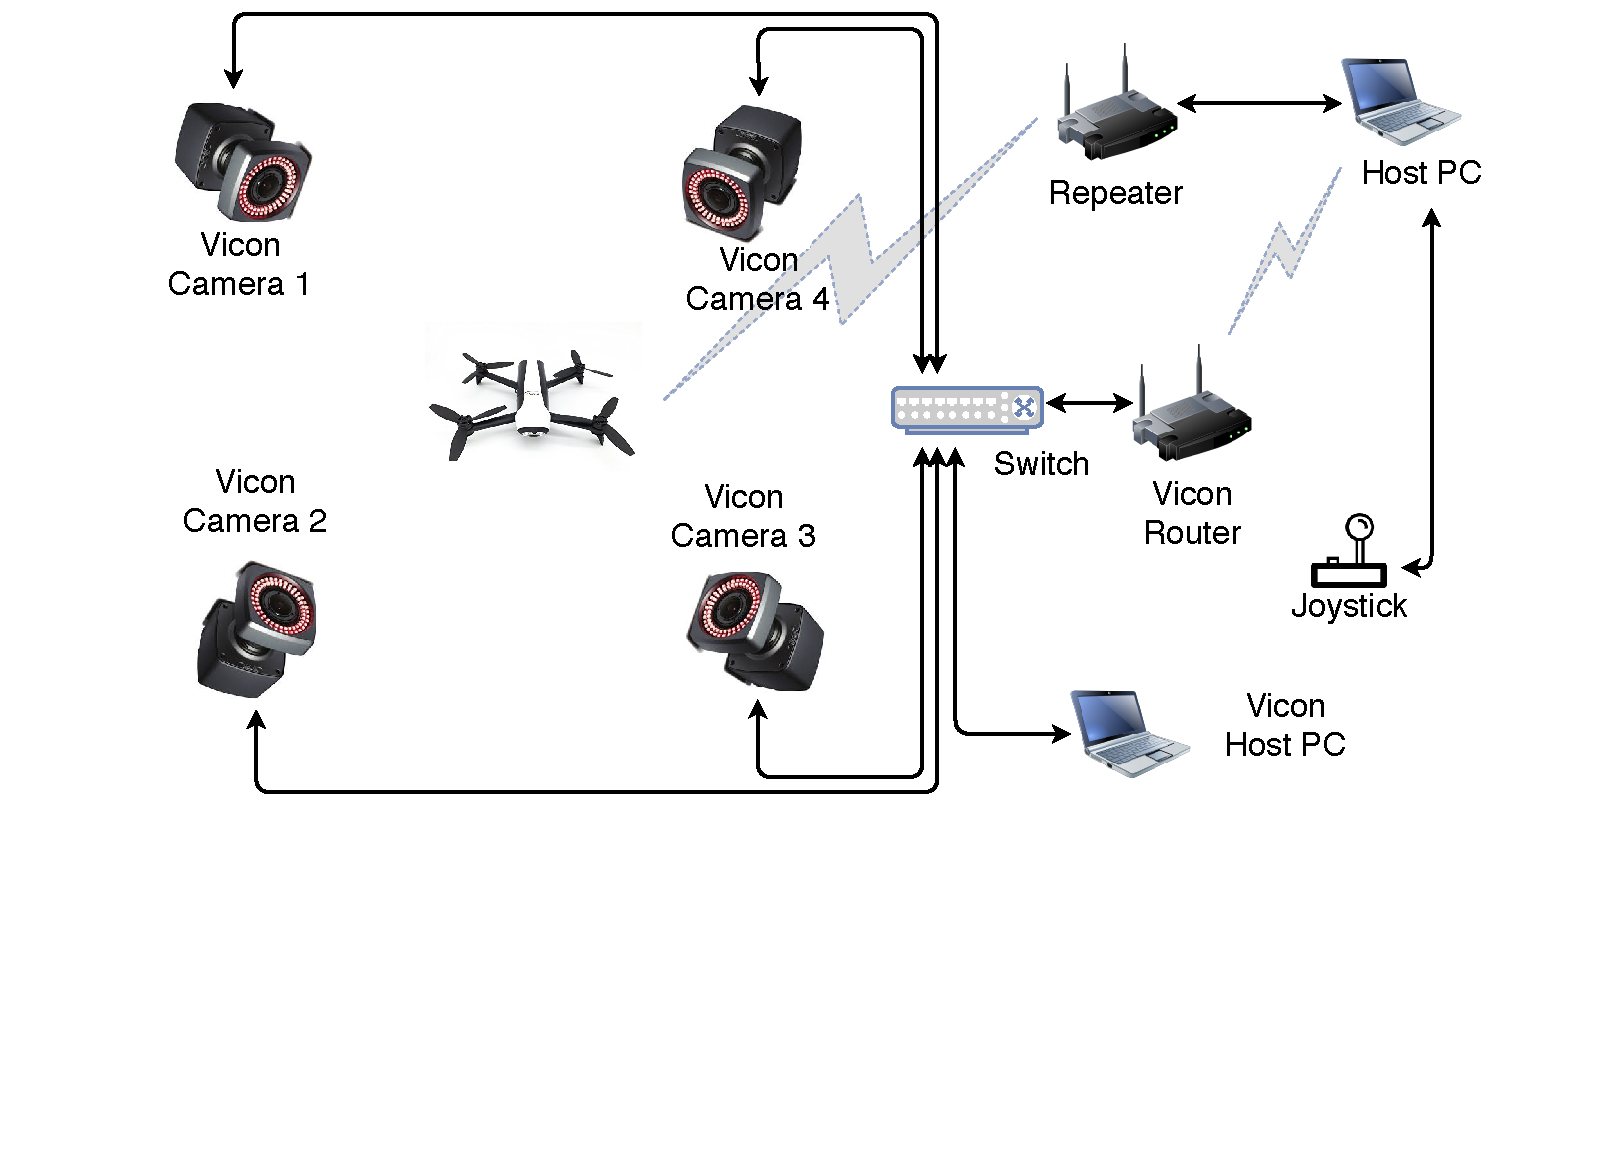
\includegraphics[scale=0.35,trim={2.5cm 6cm 1.5cm 0},clip]{img/Diagram_ViconDroneDev.pdf}
		\caption{A diagram representing the setup for an indoor flight. Source: Author (2019)}\label{fig:ViconDiagram}
	\end{figure}
\end{block}
\end{frame}